\chapter{Research and theory}
\label{research}
The first part of this chapter gives an introduction to artificial neural networks (ANNs). It begins with a definition of fundamental terms that explain the core principles of ANN. Because the research in this area is still ongoing, the more advanced techniques described here may soon be out of date or replaced by better-performing ones and therefore the theoretical background is limited only to the extent that will be relevant for the network architecture chosen at the end.

The second part presents some of the main approaches based on machine learning which were recently used by researchers to tackle the semantic segmentation problem. However, not all of them use CNN as the core algorithm. This part summarizes the key points of the corresponding papers that contributed to this topic by presenting novel architectures and principles. It concludes by a detailed description of a method that is eventually found to be the most promising and is thus selected for the final implementation.

\section{Architecture of artificial neural networks}

The inspiration for neural networks comes from their resemblance to biological neurons and the way they are connected. Neural networks can recognize features in a given training set of data and apply this knowledge to previously unseen data after the training. This strategy is called supervised learning. In supervised learning, one periodically feeds the network with input/output pairs of training data. The network learns by comparing the correct and computed output values for the given input. The network's trainable parameters are changed as the training continues to minimize the differences between network outputs and targets for \textbf{all} input patterns in the training set. \cite{mehlig}

\subsection{Feed-forward networks}

The goal of a feed-forward neural network is to find a non-linear, generally n-dimensional function that maps the space of inputs $ x $ to the space of outputs $ y $. In other words, to learn the function \cite{santiago}

\begin{gather}
f^*: \mathbb{R}^m \rightarrow \mathbb{R}^n, f^*(x;\phi)
\end{gather}

\noindent where $ \phi $ are trainable parameters of the network. The goal is to learn the value of the parameters that result in the best function approximation by solving the equation \cite{santiago}

\begin{gather}
\phi \leftarrow \, \text{arg min} \, L(y, f^*(x;\phi))
\end{gather}

\noindent where $ L $ is the loss function chosen for the particular task. One can understand the term 'loss function' simply as a metric of how happy we are about the output that the network gives us for a given input. Therefore, $f^*(x;\phi)$ is driven to match the ideal function $f(x;\phi)$ during network training. 

The structure of a feed-forward network is usually composed of many nested functions. For instance, there might be three functions $f^{(1)}$, $f^{(2)}$ and $f^{(3)}$ connected in a chain: \cite{santiago}

\begin{gather}
f(x) = f^{(3)}(f^{(2)}(f^{(1)}(x)))
\end{gather}

These models are referred to as feed-forward because information flows from the deepest nested function $f^{(1)}$ which then takes $ x $ as its direct input to other functions in the chain and finally to the output $ y $. One can name the functions starting by $f^{(1)}$ as the first layer (input layer) of the network, $f^{(2)}$ as the second layer and so on. The final layer of the network is called the output layer. \cite{santiago}

Remember that in supervised learning one needs a set of training data, in this case a set of matching $ x, y $\footnote{Outputs $ y $ are often called labels in classification tasks}  pairs. The training samples specify what the output layer must do at each point $ x $; it must produce a value that is as close as possible to $ y $. The behaviour of the other layers is not specified by the training data which is why we call these layers 'hidden layers'. \cite{santiago}

A neural network can be seen as something capable of modelling almost any function we can think of (general approximation theorem, see \cite{goodfellow}). The power of this brings us to the definition of a classification task. In this task, the function which the network approximates has discrete states (true/false in the simplest case). 

\subsection{McCulloch-Pitts neurons}

Layers of a feed-forward network further divide into distinct functions called neurons. This is where the resemblance to biological neurons comes into play: the neurons are mathematically modeled as linear threshold units (McCulloch-Pitts neurons). The output of a neuron is dependent on the output of the neurons in the previous layer. In the simplest form, the output of each neuron in the network has only two states: active or inactive. \cite{mehlig}

If the output exceeds a given threshold then the state of the neuron is said to be active, otherwise it is inactive. The model is illustrated in Figure 1.4. Neurons usually perform repeated computations in discrete time steps $ t = 0,1,2,3,.... $ The state of neuron number $ j $ at time step $ t $ is denoted by \cite{mehlig}

\begin{gather}
n_j(t) = 
	\begin{cases}	
		0 & \text{inactive,}\\
		1 & \text{active.}
	\end{cases} 
\end{gather}
\noindent Given the signals $ n_j(t+1) $, neuron number $ i $ computes \cite{mehlig}

\begin{gather}
\label{neuron_output}
n_j(t+1)=\theta_H \left(\sum\limits_{j}w_{ij}n_j(t) - \mu_i \right)
\end{gather}

As written, this computation is performed for all $ i $ neurons in parallel and the outputs $ n_i $ are the inputs to all neurons at the next time step $ t+1 $.

\newpage
\vspace{5mm}
\begin{figure}[htb]
	\begin{center}
		\includegraphics*[width=13cm, keepaspectratio]{obr/neuron.png}
	\end{center}
	\vspace{5mm}
	\caption{Schematic diagram of a McCulloch-Pitts neuron. The strength of the connection from
		neuron $ j $ to neuron $ i $ is denoted by $ w_{ij} $ \cite{mehlig}} 
	\label{neuron}
\end{figure}

Each incoming connection from other neurons has a different strength. This is determined by the parameters $ w_{ij} $ called weights . The first index $ i $ refers to the neuron whose output is being computed and $ j $ labels all neurons that connect
to neuron $ i $. The argument of $ \theta_H $ of the neuron is often referred to as the local field \cite{mehlig}

\begin{gather}
\label{local_field}
b_i = \sum\limits_{j}w_{ij}n_j(t) - \mu_i
\end{gather}

\noindent where $ b_i $ is a weighted linear average of the inputs $ n_j $ and $ \mu_i $ is an offset (threshold). Finally, the function $ \theta_H $ is referred to as the activation function. \cite{mehlig}

\subsection{Activation functions}

The general motivation for using activation functions is to bring non-linearity to the model. In the simplest case that has been discussed so far, the neurons can only have the states 0/1, which in terms of the activation function corresponds to the Heaviside function \cite{mehlig}

\begin{gather}
	\theta_H(b) = 
	\begin{cases}	
	1 & \text{for $b \geq 0$,}\\
	0 & \text{for $b < 0$.}
	\end{cases} 
\end{gather}

\noindent In practice, however, the simplest model must be generalized by allowing the neuron to respond continuously to its inputs. This is necessary for the optimization algorithms used in the training phase to operate smoothly \cite{groman}. Therefore, the term $ \theta_H $ in Eq. \eqref{neuron_output} is replaced by a general continuous activation function $ g(b) $. \cite{mehlig}

\newpage

One can choose from several activation functions which all come with their pros and cons depending on the particular application of the network. In general, there are a few requirements these functions should meet: \cite{groman}

\begin{itemize}
	
\item \textbf{Nonlinearity}. As discussed above, non-linearity is a general ability of a neural network which allows it to model very complex functions.
\item \textbf{Monotocity and nondecreasibility}. These allow certain optimization algorithms to perform with greater stability.
\item \textbf{Differentiability (or at least piecewise differentiability)}. This is useful not only in terms of stability of the optimization algorithms but also for the analytical derivation of the update rule for the network parameters during optimization. 
		
\end{itemize}

There are activation functions designed specifically for the output layer. The reason for that comes from the definition of a classification task, where we would like to interpret the outputs of the network as relative probabilities of the input belonging to a certain class. For this, the commonly-used softmax activation function can be used. We say 'relative' because the network's decision is only based on the features of one particular pattern in comparison with other data we used during training. Hence, the probabilities computed by the softmax classifier are better thought of as confidences where the ordering of the scores is interpretable, but the absolute numbers are technically not. \cite{stanford-github}

Another possibility for the output activation function is the sigmoid function, which is used for both input/hidden and output layers. Here are the most frequently used activation functions: \cite{groman}

\subsubsection{Sigmoid}
\vspace{5mm}

\begin{figure}[h]  
	\centering 
	\begin{subfigure}[b]{0.4\linewidth}
		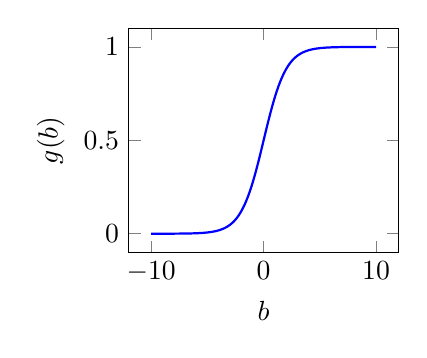
\begin{tikzpicture}
			\begin{axis}[
			scale=0.5,	
			xlabel={$ b $},
			ylabel={$ g(b) $},
			%xmin=-10, xmax=10,
			%ymin=0, ymax=1,
			%xtick={0,20,40,60,80,100},
			ytick={0, 0.5, 1},
			no markers,
			every axis plot/.append style={thick}
			]		
			\addplot[domain=-10:10,blue,samples=200]{ (1/(1 + exp(-x))) }; 				
			\end{axis}			
		\end{tikzpicture}
		\caption{$ g(b)=\frac{1}{1 + e^{-b}} $}   
	\end{subfigure}
	\begin{subfigure}[b]{0.4\linewidth}
		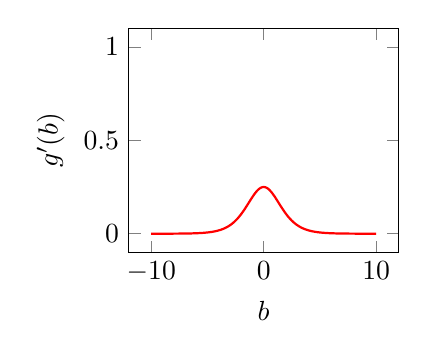
\begin{tikzpicture}
			\begin{axis}[
			scale=0.5,	
			xlabel={$ b $},
			ylabel={$ g'(b) $},
			%xmin=-10, xmax=10,
			ymin=-0.1, ymax=1.1,
			%xtick={0,20,40,60,80,100},
			ytick={0, 0.5, 1},
			no markers,
			every axis plot/.append style={thick}
			]		
			\addplot[domain=-10:10,red,samples=200]{ (1/(1 + exp(-x)))*(1-(1/(1 + exp(-x)))) }; 
			\end{axis}
		\end{tikzpicture}
		\caption{$ g'(b)=g(b)(1-g(b)) $}  
	\end{subfigure}
	\vspace{10mm}
	\caption{Sigmoid function and its derivative. Notice that the derivative goes to zero very quickly.}
\end{figure}

%\begin{minipage}{0.5\linewidth}
%	\begin{figure}		
%		
%	\caption{zdarec}
%	\end{figure}
%\end{minipage}%
%\begin{minipage}{0.32\linewidth}
%	\begin{center}	

%	\end{center}
%\end{minipage}%

This function has a clear interpretation of neuron states - active/inactive is represented by values 1/0. The sigmoid function is currently not favoured for large networks. In short, it does not have optimal properties for the learning algorithm because it saturates very quickly. Also, the fact that its mean value is non-zero doesn't have a positive impact on the learning process either. \cite{stanford-github} \cite{groman}

\subsubsection{Hyperbolic tangent}

\vspace{5mm}
\begin{figure}[h]  
	\centering 
	\begin{subfigure}[b]{0.4\linewidth}
		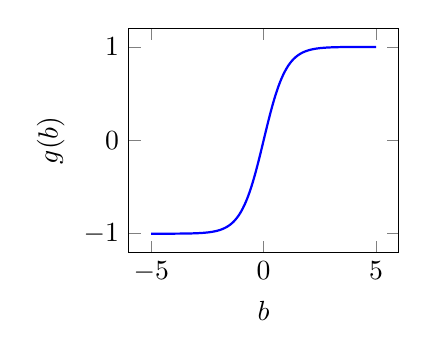
\begin{tikzpicture}
			\begin{axis}[
			scale=0.5,	
			xlabel={$ b $},
			ylabel={$ g(b) $},
			%xmin=-10, xmax=10,
			%ymin=0, ymax=1,
			%xtick={0,20,40,60,80,100},
			ytick={-1, 0, 1},
			no markers,
			every axis plot/.append style={thick}
			]		
			\addplot[domain=-5:5,blue,samples=200]{tanh(x)}; 
			\end{axis}
		\end{tikzpicture}
		\caption{$ g(b)=\tanh(b) $}   
	\end{subfigure}
	\begin{subfigure}[b]{0.4\linewidth}
		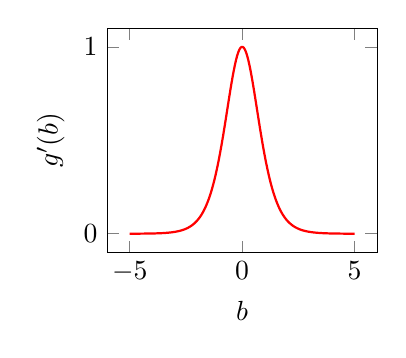
\begin{tikzpicture}
			\begin{axis}[
			scale=0.5,	
			xlabel={$ b $},
			ylabel={$ g'(b) $},
			%xmin=-10, xmax=10,
			%ymin=0, ymax=1,
			%xtick={0,20,40,60,80,100},
			ytick={-1, 0, 1},
			no markers,
			every axis plot/.append style={thick}
			]		
			\addplot[domain=-5:5,red,samples=200]{1-tanh(x)*tanh(x)}; 
			\end{axis}
		\end{tikzpicture}
		\caption{$ g'(b)=1-\tanh^2(b) $}  
	\end{subfigure}
	\vspace{10mm}
	\caption{Hyperbolic tangent and its derivative.}
\end{figure}

Unlike the sigmoid function, the range of its output is in the interval <-1,1> and the output is therefore zero-centered. In practice, the tanh non-linearity is always preferred to the sigmoid non-linearity. \cite{stanford-github}

\subsubsection{Rectified linear unit (ReLu)}
\vspace{5mm}

\begin{figure}[h]  
	\centering 
	\begin{subfigure}[b]{0.4\linewidth}
		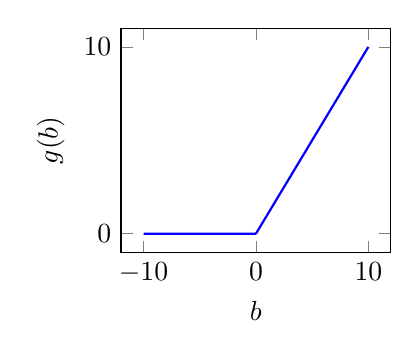
\begin{tikzpicture}
			\begin{axis}[
			scale=0.5,	
			xlabel={$ b $},
			ylabel={$ g(b) $},
			%xmin=-10, xmax=10,
			%ymin=0, ymax=1,
			%xtick={0,20,40,60,80,100},
			ytick={ 0, 10},
			no markers,
			every axis plot/.append style={thick}
			]		
			\addplot[domain=-10:10,blue,samples=200]{max(0,x)}; 
			\end{axis}
		\end{tikzpicture}
		\caption{$ g(b)=\max(0,x) $}   
	\end{subfigure}
	\begin{subfigure}[b]{0.4\linewidth}
		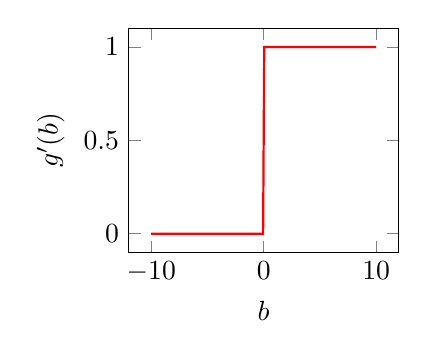
\begin{tikzpicture}
			\begin{axis}[
			scale=0.5,	
			xlabel={$ b $},
			ylabel={$ g'(b) $},
			%xmin=-10, xmax=10,
			%ymin=-0.1, ymax=10.1,
			%xtick={0,20,40,60,80,100},
			%ytick={ 0, 10},
			no markers,
			every axis plot/.append style={thick}
			]		
			\addplot[domain=-10:10,red,samples=200]{(sign(x)+1)/2}; 
			\end{axis}
		\end{tikzpicture}
		\caption{$ g'(b)= \theta_H (x) $}  
	\end{subfigure}
	\vspace{10mm}
	\caption{ReLu and its derivative. ReLu does not saturate!}
\end{figure}

The authors of this function found the inspiration in real biological neurons: there is a threshold below which the response of the neuron is strictly zero, as shown in the figure above. The derivative of the ReLU function is discontinuous at $ x=0 $. A common convention is to set the derivative to zero at $ x=0 $. It is now the standard function to use in large networks for image recognition. \cite{mehlig}

\newpage

\subsubsection{Leaky ReLu}
\vspace{3mm}
\begin{figure}[h]  
	\centering 
	\begin{subfigure}[b]{0.4\linewidth}
		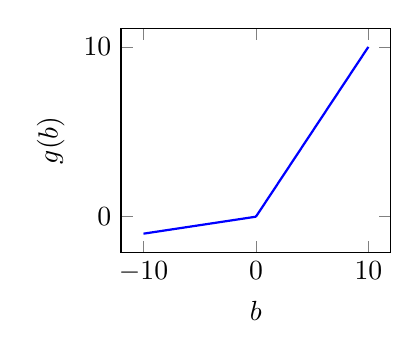
\begin{tikzpicture}
		\begin{axis}[
		scale=0.5,	
		xlabel={$ b $},
		ylabel={$ g(b) $},
		%xmin=-10, xmax=10,
		%ymin=0, ymax=1,
		%xtick={0,20,40,60,80,100},
		ytick={ 0, 10},
		no markers,
		every axis plot/.append style={thick}
		]		
		\addplot[domain=-10:10,blue,samples=200]{max(x,0.1*x)}; 
		\end{axis}
		\end{tikzpicture}
		\caption{$ g(b)= 
			\begin{cases}	
			b & \text{for $b \geq 0$,}\\
			0.01b & \text{for $b < 0$.}
			\end{cases}  $}    
	\end{subfigure}
	\begin{subfigure}[b]{0.4\linewidth}
		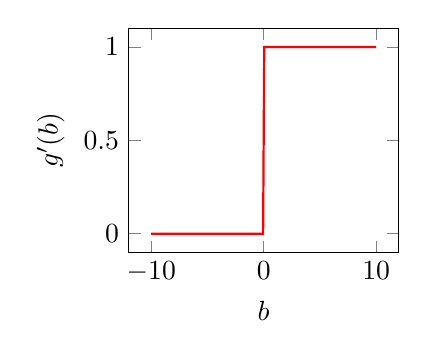
\begin{tikzpicture}
		\begin{axis}[
		scale=0.5,	
		xlabel={$ b $},
		ylabel={$ g'(b) $},
		%xmin=-10, xmax=10,
		%ymin=-0.1, ymax=10.1,
		%xtick={0,20,40,60,80,100},
		%ytick={ 0, 10},
		no markers,
		every axis plot/.append style={thick}
		]		
		\addplot[domain=-10:10,red,samples=200]{(sign(x)+1)/2}; 
		\end{axis}
		\end{tikzpicture}
		\caption{$ g'(b)= 
			\begin{cases}	
			1 & \text{for $b \geq 0$,}\\
			0.01 & \text{for $b < 0$.}
			\end{cases}  $}  
	\end{subfigure}
	\vspace{10mm}
	\caption{Leaky ReLu and its derivative.}
\end{figure}

By modifying the previously introduced function one gets a version of ReLu intended to address its biggest drawback, which is the fact that some neurons may become dead (their output will be always zero) and thus they do not contribute to the network's output. Unfortunately, there's generally no guarantee that using Leaky ReLu instead of ReLu will always yield better results. \cite{stanford-L4}

\newpage

\subsection{Multilayer perceptrons}

Perceptron is a feed-forward network. It is divided into layers consisting of McCulloch-Pitts neurons. The left-most layer of the network shown in Figure \ref{perceptron} is called input layer. The input layer takes the values of the input data and passes it to the next layer. The right-most layer is the output layer where the output of the network is read out. The other neuron layers are called hidden layers; their states are not read out directly. \cite{mehlig}

\vspace{3mm}
\begin{figure}[htb]
	\begin{center}
		\includegraphics*[height=6cm, keepaspectratio]{obr/perceptron.png}
	\end{center}
	\vspace{3mm}
	\caption{Perceptron with one hidden layer. \cite{mehlig}} 
	\label{perceptron}
\end{figure}

\textquote{\textit{In perceptrons, all connections (called weights) $ w_{ij} $ are one-way. Every neuron (or input terminal) feeds only to neurons in the layer immediately to the right. There are no connections within layers, or back connections, or connections that jump over a layer. There are $ N $ input terminals.}} \cite{mehlig} We denote the inputs coming to the input layer by \cite{mehlig}

\begin{gather}
	x(\mu)= 
	\begin{bmatrix}
	x_{1}^{(\mu)} \\
	x_{2}^{(\mu)} \\
	\vdots \\
	x_{N}^{(\mu)} 
	\end{bmatrix}
\end{gather}

The index $ \mu $ labels different input patterns in the training set. The perceptron in Figure \ref{neuron} calculates the output as follows: \cite{mehlig}

\begin{gather}
V_j^{(\mu)} = g(b_j^{(\mu)}) \quad \text{where} \quad b_j^{(\mu)} = \sum_{k} w_{jk} x_{k}^{(\mu)} - \theta_{j} \\
O_i^{(\mu)} = g(B_i^{(\mu)}) \quad \text{where} \quad B_i^{(\mu)} = \sum_{j} W_{ij} V_{j}^{(\mu)} - \Theta_{i} 
\end{gather}

Here $ V_j^{(\mu)} $ denotes the output of hidden layer $ j $ based on the local field $ b_j^{(\mu)} $ and activation function $ g(b) $. The parameters $ w_{jk} $ and $ \theta_{j} $ denote weights and thresholds of the layer $ j $. Corresponding computations are made for the output layer whose parameters are denoted by capital letters. \cite{mehlig} A multilayer perceptron generally has $ N $ hidden layers. If it has more than two hidden layers, it usually begins to be called a deep network. 

\subsubsection{Output classifier - softmax}

The softmax function is designed to be used in output layers. This so-called 'classifier' differs from other activation functions by its dependency on other neurons in the layer \cite{mehlig}

\begin{gather}
O_{i} = \frac{e^{\alpha b_i^{(L)}}}{\sum_{k=1}^{M} e^{\alpha b_k^{(L)}}}
\end{gather}

\enquote{\textit{Here $ b_{i}^{(L)} = \sum_{j}w_{ij}^{(L)} V_{j}^{(L-1)} - \theta _{j}^{(L)} $  are the local fields of the neurons in the output layer $ L $. The constant $\alpha$ is usually taken to be unity. Softmax has three important properties: first that $ 0 \geq O_i \geq 1 $. Second, the values of the outputs sum to one $ \sum_{i=1}^{M} O_i = 1 $. This means that the outputs of Softmax units can be interpreted as probabilities. Third, the outputs are monotonous: when $ b_i^{(L)} $ increases, then $ O_i $ increases but the values $ O_k $ of the other output neurons $ k \neq i $ decrease.}} \cite{mehlig}

\vspace{3mm}
\begin{figure}[htb]
	\begin{center}
		\includegraphics*[width=3.4cm, keepaspectratio]{obr/softmax.png}
	\end{center}
	\vspace{3mm}
	\caption{Softmax classifier: the neurons in this layer are
		not independent. \cite{mehlig}} 
	\label{softmax}
\end{figure}

\subsubsection{Linear separability}

The reason we use hidden layers is to tackle classification problems that are not linearly separable. Linear separability is shown in Figure \ref{separability}, where the input to the network is two-dimensional. We classify the input data into two classes (marked as black and white points in the graph). \cite{mehlig}

\begin{figure}[htb]
	\begin{center}
		\includegraphics*[width=11cm, keepaspectratio]{obr/separability.png}
	\end{center}
	\vspace{3mm}
	\caption{Linearly separable (left) and not linearly separable problems (right). The decision boundary needs to be piece-wise linear for the not linearly separable problem \cite{mehlig}} 
	\label{separability}
\end{figure}

A classification problem is linearly separable if one is able to draw a single line (a single plane in case of three inputs, etc.) to divide the input space into two distinct areas. The curve that separates the space of inputs is called the decision boundary. The position of the decision boundary is determined by the values of weights and thresholds of the neurons. These parameters are found by training the network. In the case shown in Figure \ref{separability} (left), the line dividing the 2D space of inputs corresponds to the simplest possible case which is a single neuron in the network. In a not linearly separable task (Figure \ref{separability}, right) we need to divide the input space into more than two regions to solve the classification. By doing this, we map the input space of size n = 2 to the hidden space of size m = 3 and use it as an input to other layers. \cite{mehlig}

%-------------------TRAINING----------------------

\newpage

\section{Training of artificial neural networks}

Artificial neural networks are trained using iterative optimization algorithms. During training, one needs to choose the right loss function whose value goes to zero when the network produces the expected output. To achieve this, trainable paremeters are changed in each step of optimization. The effect each parameter has on the value of the loss function is determined by calculating the gradient of the loss function with respect to the particular parameter in the network. The way this information is used is then subject to the chosen algorithm. \cite{notes}

\subsection{Loss function}

Loss function is a metric of our satisfaction with the network's output. The choice depends on the nature of the task that the network is used for and on the activation function used in the output layer. During training, the loss function is the one whose value is being optimized. Here are the most commonly used functions: \cite{mehlig}


\subsubsection{Mean Squared Error (MSE)}

\begin{gather}
	L =  \frac{1}{2} \sum\limits_{\mu i} \left( t_{i}^{(\mu)} - O_{i}^{(\mu)} \right)^2
\end{gather}

MSE is used for regression tasks, often in combination with the sigmoid function in the output layer. \cite{groman}

\subsubsection{Negative Log Likelihood} 

\begin{gather}
	L = - \sum\limits_{\mu i}  t_{i}^{(\mu)} \ln (O_{i}^{(\mu)})
\end{gather}

The negative log likelihood is used for classification tasks in combination with the softmax classifier. \cite{mehlig}

\subsubsection{Cross Entropy Loss} 

\begin{gather}
	L = - \sum\limits_{\mu i}  t_{i}^{(\mu)} \ln (O_{i}^{(\mu)}) + (1 - t_{i}^{(\mu)}) \ln (1 - (O_{i}^{(\mu)}))
\end{gather}

Very similar to the negative log likelihood loss. The difference is that it works with the sigmoid activation function. \cite{mehlig}

\newpage
\subsection{Gradient optimization and backpropagation}

Backpropagation is a way in which information about the correctness of the output flows through the network so that the parameters in all layers can be adjusted. Everytime we feed the network with an input pattern $ \mu $ we get the output values of the neurons in all layers. This is called a forward pass (inference, left-to-right pass). Then we want to evaluate the correctness of the output and pass that information back to the network. The second phase is called backpropagation because the error propagates from the output layer to the layers on the left. \cite{mehlig}

\vspace{3mm}
\begin{figure}[htb]
	\begin{center}
		\includegraphics*[width=4.2cm, keepaspectratio]{obr/backpropagation.png}
	\end{center}
	\vspace{3mm}
	\caption{Backpropagation algorithm: the states of the neurons are updated forward
		(from left to right) while errors are updated backward (right to left) \cite{mehlig}} 
	\label{backprop}	
\end{figure}

%_____FILIPEK REWRITE_____

The optimization algorithm searches the most optimal value of the loss function whose value is dependent on the trainable parameters. For this, the algorithms needs to move in the direction of the steepest descent in the landscape of the loss function. In each step of the optimization, one needs to calculate partial derivatives of the loss function with respect to all trainable parameters. The derivative is found by applying the chain rule to the formula for calculating the loss function. \cite{mehlig}

\subsubsection{Gradient descent}

The general formula for the gradient descent algorithm goes as follows: \cite{notes}

\begin{gather}
	\delta \phi = - \eta \frac{\partial L}{\partial \phi}
\end{gather}

\noindent where $ \phi $ is the parameter we care about (weights, thresholds, etc.) and $ L $ is the loss function. Parameter $ \eta $ is called the learning rate. This parameter determines the size of the step we take in the way of the steepest descent in the loss function's landscape (in the case of two parameters). \cite{notes}

Figure \ref{learning_rate} shows that the choice of the learning rate value has a strong effect on the course of the optimization and the convergence of the algorithm. If the steps are too small, the training will be slow and the algorithm is prone to getting stuck in local minima. On the other hand, if the value of it is too big, the algorithm may even start to 'climb up the hill' and cause the loss function to grow. \cite{mehlig} 

\newpage

\vspace{3mm}
\begin{figure}[htb]
	\begin{center}
		\includegraphics*[width=14cm, keepaspectratio]{obr/learning_rate.png}
	\end{center}
	\vspace{3mm}
	\caption{Effect of the learning rate on optimization: the value must be chosen carefully for the algorithm to converge. \cite{coors}} 
	\label{learning_rate}
\end{figure}

Given a multilayer perceptron with hidden layers and their parameters $ w_{mn}, \theta_m $, output layer with weights $ W_{mn}, \Theta_m $ and the MSE loss function, the gradient descent algorithm gives the weight updates in the form \cite{mehlig}

\begin{gather}
	\delta W_{mn} = - \eta \frac{\partial L}{\partial W_{mn}} = \eta \sum\limits_{\mu=1}^{p}
	(t_{m}^{(\mu)} - O_{m}^{(\mu)})   g'(B_{m}^{(\mu)})     V_{n}^{(\mu)}
\end{gather}

\noindent where $ p $ is the total number of training samples, $ V_{n}^{(\mu)} $ is the vector of outputs of neurons in the previous layer $ n $ for the sample $ \mu $. For clarity, one usually defines the 'weighted error' as \cite{mehlig}

\begin{gather}
	\Delta_{m}^{(\mu)} = (t_{m}^{(\mu)} - O_{m}^{(\mu)})   g'(B_{m}^{(\mu)})
\end{gather}

\noindent The update rules for hidden layers are also obtained by using chain rule, which gives \cite{mehlig}

\begin{gather}
\delta w_{mn} = - \eta \frac{\partial L}{\partial w_{mn}} = \eta \sum\limits_{\mu=1}^{p} \sum\limits_{i=1}^{N}
\Delta_{i}^{(\mu)} W_{im} \, g'(b_{m}^{(\mu)}) x_{n}^{(\mu)}
\end{gather}

\noindent while putting \cite{mehlig}

\begin{gather}
\delta_{m}^{(\mu)} = \sum\limits_{i=1}^{N} \Delta_{i}^{(\mu)} W_{im} \, g'(b_{m}^{(\mu)})
\end{gather}

\noindent Putting all the above together gives \cite{mehlig}

\begin{gather}
\label{update_rule}
\delta w_{mn} = \eta \sum\limits_{\mu=1}^{p} \delta_{m}^{(\mu)} x_{n}^{(\mu)}
\quad \text{and} \quad 
\delta W_{mn} = \eta \sum\limits_{\mu=1}^{p} \Delta_{m}^{(\mu)} V_{n}^{(\mu)}	
\end{gather}

\noindent Similarly, we get the update rule for thresholds (see \cite{mehlig}). In summary, the steps of backpropagation + gradient descent are the following: \cite{mehlig}
\vspace{5mm}
\begin{algorithm}
	\caption{Gradient descent \cite{mehlig}}
	\begin{algorithmic}[1]
		\item Pick input pattern $ \mu $ from the training set and perform forward pass
		\item Compute errors $ \Delta_{m}^{(\mu)} $ for output layer
		\item Compute errors $ \delta_{m}^{(\mu)} $ for hidden layers
		\item Perform updates $w_{mn} = w_{mn} + \delta w_{mn} \quad \text{and} \quad \theta_{mn} = \theta_{mn} + \delta \theta_{mn}$, the same for the output layer
	\end{algorithmic}
\end{algorithm}

\subsubsection{Stochastic gradient descent}

Gradient methods are generally prone to getting stuck in local minima of the optimized function. The way to adress this is to add a little bit of noise to the process. In stochastic gradient descent, this is achieved by summing over smaller portions of the training data rather than over the entire dataset. These portions of the data are called mini-batches. \cite{mehlig} \\

In Equations \ref{update_rule} we see that in each iteration one needs to sum overall training patterns in the set to obtain the value of the gradient. In stochastic gradient descent (SGD), one only sums over randomly chosen $ mb $ patterns from the training set and then immediately performs the weight update. The process is repeated until all training data have been used (this is called a training epoch). In mini-batches, samples appear only once per epoch and the entire training set is usually shuffled after each epoch. \cite{mehlig} Applying the above, the Equations \ref{update_rule} slightly change to \cite{mehlig}

\begin{gather}
\delta w_{mn} = \eta \sum\limits_{\mu=1}^{mb} \delta_{m}^{(\mu)} x_{n}^{(\mu)}
\quad \text{and} \quad 
\delta W_{mn} = \eta \sum\limits_{\mu=1}^{mb} \Delta_{m}^{(\mu)} V_{n}^{(\mu)}	
\end{gather}

\subsubsection{Vanishing and exploding gradient problems}

When we compute the weight increments using MSE, the further from the output layer we go, the more the term $ g'(b) $ accumulates (with each next layer). The point is that MSE is often used with the sigmoid activation functions whose derivative drops to a small number in its area of saturation resulting in very small weight increments. This phenomenon is known as the vanishing gradient problem \cite{mehlig}. Similarly, one can run into trouble when the values of the derivative of activation function are larger than one. Then the value of the gradients may start growing exponentially: this is called the exploding gradient problem. \cite{eniola} One of the ways to address these problems is using activation functions that do not saturate (ReLu, Leaky ReLu, etc.). \cite{mehlig} \cite{stanford-L4}

\subsubsection{Momentum}

There are several ways to make the stochastic gradient descent algorithm perform better. The key is to prevent it from getting stuck in local minima. Gradient methods also tend to slow down in the areas of minima that are very shallow. The obvious solution to this is to take bigger steps by using a larger value of the learning rate. This can, however, make the algorithm oscillate. \cite{mehlig} One way to tackle this is to implement the mechanism fittingly called momentum. 

When using momentum, we can imagine that the SGD algorithm behaves like a ball that rolls downhill and develops speed over time \cite{stanford-L7}. The resulting move made by the algorithm in the landscape of the loss function is, therefore, a combination of the gradient vector and the velocity vector. The update rule for weights gets modified to \cite{mehlig}

\begin{gather}
\delta w_{ij}^{(t)} = - \eta \frac{\partial L}{\partial w_{ij}^{(t)}} + \alpha \delta w_{ij}^{(t-1)} 
\end{gather}

\noindent where $ t=0,1,2,..,n $ is the iteration number and $ \delta w_{ij}^{(0)} = \partial L / \partial w_{ij}^{(0)} $ is the weight increment in the zeroth time step. The parameter $ \alpha > 0$ is the momentum constant. 

There are other ways of implementing momentum, such as the commonly used Nesterov's accelerated gradient method (see \cite{mehlig} \cite{stanford-github} for details). This algorithm differs from the simple momentum by altering the steps the algorithm takes to do the final update: it first moves in the direction of the velocity, then evaluates the gradient at that point and corrects the previous step. It turns out that this method performs better in practice \cite{stanford-L7}.

%https://www.deeplearningbook.org/ Googfellow

\vspace{4mm}
\begin{figure}[htb]
	\begin{center}
		\includegraphics*[width=12cm, keepaspectratio]{obr/momentum.png}
	\end{center}
	\vspace{4mm}
	\caption{Momentum (left) and Nesterov's Momentum (right). \cite{mehlig}} 
	\label{momentum}
\end{figure}

\newpage
\subsubsection{Other optimization algorithms}

The algorithms below extend the idea of stochastic gradient descent by introducing various strategies of learning rate adaptation during training. In most cases, using more advanced algorithms tends to speed up the training and usually helps finding more optimal parameters in terms of the loss value. 

\begin{itemize}
	\item \textbf{AdaGrad}
	
	AdaGrad is another gradient based algorithm. In the previously discussed gradient descent, the parameters were updated with the same learning rate in every step of the algorithm. AdaGrad adapts the learning rate based on the accumulated square of gradients (see \cite{stanford-L7}). The problem is that it might get stuck in the saddle points beacause the size of the steps it takes gets very small as the training goes on. \cite{stanford-L7}
	
	\item \textbf{AdaDelta and RMSprop}
	
	These algorithms are an extension of AdaGrad and tackle its tendency to drop some of the learning rates to almost infinitely small values. They were published simultaneously but independently of one another. \cite{groman}
	
	\item \textbf{Adam}
	
	Adam can be seen as a combination of RMSprop and Stochastic Gradient Descent with momentum. It uses squared gradients to scale the learning rate like RMSprop and it takes advantage of momentum by using a moving average of the gradient instead of the gradient itself like SGD with momentum. \cite{bushaev} \cite{groman}

\end{itemize}

	\vspace{4mm}
\begin{figure}[htb]
	\begin{center}
		\includegraphics*[width=11cm, keepaspectratio]{obr/opt.png}
	\end{center}
	\vspace{4mm}
	\caption{Comparison of different optimization algorithms. \cite{groman}} 
	\label{algorithms}
\end{figure}

\newpage
\subsection{Improving training performance}
\subsubsection{Initialization of weights and thresholds}

The standard approach is to initialise the weights to independent Gaussian random numbers with mean zero and unit variance and to set the thresholds to zero. But in networks that have large hidden layers with many neurons, this scheme may fail. This is because the variance of weights is not taken care of, which leads to very large (or small) activation values, resulting in exploding (or vanishing) gradient problem during backpropagation. \cite{mehlig} Here are some of the more advanced initialization methods:

\begin{itemize}
	\item \textbf{Xavier initialization}
		
	Xavier initialization sets the layer’s weights to values from the Gaussian distribution. The mean and standard deviation are determined by the number of incoming and outcoming network connections to the layer. These random numbers are then divided by the square root of the number of incoming connections. This method works well with the tangent and sigmoid activation functions but fails when using ReLUs. \cite{stanford-L6}
	
	\item \textbf{MSRA initialization}

	This method differs from Xavier only in its use of a different factor to scale the Gaussian distributed numbers. It turns out that this small change works much better when using ReLU activation function. \cite{stanford-L6}
	
\end{itemize}

\subsubsection{Overfitting and regularization}

\enquote{\textit{A network with more neurons may classify the training data better because it accurately represents all specific features of the data. But those specific properties could look quite different in new data. As a consequence, we must look for a compromise between the accurate classification of the training set and the ability of the network to generalise. This problem is called overfitting: the network fits too fine details that have no general meaning.}} \cite{mehlig} The terms below are referred to as the L1 and L2 regularizations. Adding these terms to the loss function prevents the weight from growing. When the value of the weights gets very high, the local fileds of the neurons become very large too. In that case, some activation functions, like the sigmoid function or \textit{tanh}, reach their maxima very quickly which causes the vanishing gradient problem. The formulas for L1 and L2 regularizations are: \cite{mehlig}

\begin{gather}
	R_{L2}(w) = \frac{\gamma}{2} \sum\limits_{ij} w_{ij}^{2} \quad \text{or} \quad R_{L1}(w) = \frac{\gamma}{2} \sum\limits_{ij} |w_{ij}|
\end{gather}

\enquote{\textit{These two regularization schemes tend to help against overfitting. (...) Weight decay dds a constraint to the problem of minimising the energy function. When the weights are small, then small changes in some of the patterns do not give a substantially different training result. When the network	has large weights, by contrast, it may happen that small changes in the input give	significant differences in the training result that are difficult to generalise.}} \cite{mehlig}

\subsubsection{Batch Normalisation}

The idea of batch normalisation is to shift and normalise the input data for each
hidden layer so that the distribution of its inputs becomes Gaussian. The values of mean and variance are computed during each forward pass (pass of a single mini-batch) and then applied to each neuron in the layer. The mean and variance are multiplied by trainable factors, usually called $ \beta, \gamma $. \cite{stanford-L6} \cite{mehlig} When the training is done, the values of $ \beta, \gamma $ for each layer are re-computed using the mean and variance of the entire training dataset and no longer change. \cite{issue}

\enquote{\textit{Batch normalisation helps to combat the vanishing-gradient problem because it prevents local fields of hidden neurons to grow. This makes it possible to use sigmoid functions in deep networks, because the distribution of inputs remains normalised. (...) It is an empirical fact that batch normalisation often speeds up the training.}} \cite{mehlig}

\subsubsection{Dropout}
\label{dropout_sec}

Dropout is a very simple scheme that helps against overfitting. During training, a random portion of neurons in the network is ignored for each input pattern/mini-batch with the probability of $ p $. This can be thought of as making the network adapt to the sparsity of the remaining neurons and making their effect on the output spread equally over the network. Another interpretation is that we are training different net architectures at the same time. When the training is done, the output of each neuron is multiplied by the probability $ p $ of a neuron being dropped out during training (weight averaging). \cite{mehlig} \cite{stanford-L7}

\vspace{4mm}
\begin{figure}[htb]
	\begin{center}
		\includegraphics*[width=11cm, keepaspectratio]{obr/dropou.png}
	\end{center}
	\vspace{4mm}
	\caption{ANN without (left) and with dropout (right). \cite{arvi}} 
	\label{dropout}
\end{figure}

\subsubsection{Data augmentation}

The general rule is that the bigger the training dataset, the better the network generalises. However, expanding a dataset manually can be very expensive. This leads to the idea of expanding it artificially. In image classification tasks, this can be done by randomly cropping, scaling, shifting and mirroring the data. \cite{mehlig}

\subsubsection{Early stopping}

\enquote{\textit{One way of avoiding overfitting is to use cross validation and early stopping. One splits the training data into two sets: a \textbf{training set} and a \textbf{validation set}. (...) The network is trained on the training set. During training, one monitors not only the energy function for the training set, but also the energy function evaluated on the validation data. As long as the network learns general features of the input distribution, both training and validation energies decrease. But when the network starts to learn specific features of the training set, then the validation energy saturates, or may start to increase. At this point the training should be stopped.}} \cite{mehlig}

When the training is done, the performance is measured using a set of 'unseen' data: the \textbf{test set}. \cite{mehlig}

\vspace{4mm}
\begin{figure}[htb]
	\begin{center}
		\includegraphics*[width=9cm, keepaspectratio]{obr/early.png}
	\end{center}
	\vspace{4mm}
	\caption{Progress of training and validation losses. The plot is schematic, and
	the data is smoothed. The training is stopped when the validation energy begins to
	increase. \cite{mehlig}} 
	\label{}
\end{figure}

\subsubsection{Transfer Learning}

To create a well-generalising neural network, one need to have access to a dataset of a sufficient size. Therefore in practice, it is unusual to train an entire CNN from scratch (with random initialization). Instead, it is common to pretrain a CNN on a very large dataset (e.g. ImageNet) and then use the CNN either as an initialization or a fixed feature extractor for the task of interest. \cite{stanford-L7}

One strategy here is to fine-tune the weights of the pretrained network by continuing backpropagation. It is possible to keep some of the earlier layers fixed and only fine-tune some higher-level portion of the network. This is motivated by the observation that the earlier features of a CNN contain more generic features (e.g. edge detectors) and the later layers become progressively focused on the details. It is common to use a smaller learning rate for CNN weights that are being fine-tuned, in comparison to the randomly-initialized weights. This is because we expect that the CNN weights already perform well and hence distorting them is not desirable. \cite{stanford-L7} \cite{stanford-github}

\subsubsection{Data pre-processing}

For most cases, it is advisable to shift the data so it has a zero mean before the training begins. When classifying images, for example, there are two ways of doing this: first, by subtracting the mean image (image of size MxNx3 for RGB) from the entire dataset or, to subtract the so-called per-channel mean (three numbers in total). The motivation behind this is the following: if we think of adjusting the weights in the network as moving the decision boundary (Figure \ref{separability} (left)), it is intuitive that the data which is not distributed around the origin will cause the classification success to get very sensitive to weight changes.\footnote{Weights in Figure \ref{separability} are the parameters that determine the slope of the decision boundary} \cite{stanford-L4} Sometimes it is also appropriate to scale the data so it has the same variance in all directions. See \cite{mehlig} for more details and other techniques.